\documentclass[a4paper,12pt]{report}
\usepackage[left=0.75in,right=0.75in,top=1.5in,bottom=1.5in,footskip=.25in]{geometry}
\usepackage{graphicx}
\usepackage[english]{babel}
\usepackage[utf8x]{inputenc}
\usepackage{url}
\usepackage[toc,automake,acronym]{glossaries}
\usepackage[section]{placeins} %This package prevents images to shift to other sections.

\newcommand{\TermName}{FALL 2019}
\newcommand{\Title}{}
\newcommand{\Course}{\textbf{SOEN-6481 \vspace{0.5cm} SOFTWARE SYSTEMS REQUIREMENTS SPECIFICATION}}
\newcommand{\ProfessorName}{Dr. PANKAJ KAMTHAN}
\setcounter{chapter}{1}




%---------------------------------------------------------------------------------------
%  GLOSSORY
%---------------------------------------------------------------------------------------

\newglossaryentry{igo}
{
	name=iGo,
	description={The online Ticket Vending Machine Web Application integrating with STM system}
}
\newglossaryentry{tvm}
{
	name=TVM,
	description={The online Ticket Vending Machine Web Application integrating with STM system}
}


\newglossaryentry{opus}
{
	name=OPUS,
	description={The online Ticket Vending Machine Web Application integrating with STM system}
}
\newglossaryentry{rechargable_card}
{
	name=Rechargable Card,
	description={A card that can be recharged to be used monthly, weekly.}
}
\newglossaryentry{non_rechargable_card}
{
	name=Non-Rechargable Card,
	description={One time use and throw card.}
}
\newglossaryentry{administrator}
{
	name=Administrator,
	description={The account to manage and administor system.}
}
\newglossaryentry{registration}
{
	name=Registration,
	description={Creating a account for new/first time user.}
}
\newglossaryentry{reduced_fare}
{
	name=Reduced Fare,
	description={Fare offered at reduced rates that the normal prices for certain users that qualify for it.}
}
\newglossaryentry{regular_fare}
{
	name=Regular Fare,
	description={Normal Fare Prices.}
}
\newglossaryentry{transaction}
{
	name=Transaction,
	description={A digital record is generated when user interacts with the system.}
}
\newglossaryentry{authentication_gateway}
{
	name=Authentication Gateway,
	description={A third party authentication system to validate users Credit/Debit cards.}
}
\newacronym{stm}{STM}{Société de transport de Montréal}

\makeglossary

\begin{document}

%----------------------------------------------------------------------------------------
%	TITLE PAGE START
%----------------------------------------------------------------------------------------

\begin{titlepage}
\newcommand{\HRule}{\rule{\linewidth}{0.5mm}} %New command for thickness of line	


\centering
\textbf{\LARGE  Concordia University} \\ [5mm] 

\includegraphics[scale=.1]{University_logo.jpg}\\[1cm] 
\textsc{\Large \Course} \\ [0.5cm]

%--------
%	TITLE
%--------
	
\HRule \\[0.4cm]
{ \huge \bfseries TICKET VENDING MACHINE \\ [5mm]  (\TermName)}\\[0.4cm] 
%{\large \textbf{DELIVERABLE 1 (D1)} }	
\HRule \\[1.5cm]


%---------
%	TAIL SECTION OF TITLE PAGE
%---------
\vspace{4cm}

\begin{flushleft}


\textbf{\underline{\Large Submitted By: (Team E)}}
\hfill
\textbf{\underline{\Large Submitted To:}} \\
\vspace{3mm}
\large Bhavpreet Kaur (40071697)
\hfill
\large Prof. Pankaj Kamthan \\

\large Navjot Kaur (40078155) \hfill \\
\large Mehrnaz Keshmirpour (40063320) \hfill \\
\large Shruthi Kondapura Venkataiah (40091427) \hfill \\
\large Sanchit Kumar (40081187	) \\

\end{flushleft}

\vspace{1.5cm}
{\large \today}\\[2cm]

\vfill
\end{titlepage}


%---------
%	TABLE OF CONTENT PAGE
%---------

\newpage

\tableofcontents



%---------
%	NEW PAGE
%---------

\chapter*{\centering Deliverable - 1}

\section{Problem 1}

\subsection{iGo Description}
The product \gls{igo} is a software solution for \gls{tvm} (Ticket Vending Machine) which allows user to purchase tickets, recharge their \gls{opus} card and get information about the different tickets \gls{stm}(Société de transport de Montréal) offers. iGO products is designed to server people in Montreal, Quebec, Canada who use STM metros and buses. STM offers two ticketing methods: \gls{rechargable_card} OPUS Card and \gls{non_rechargable_card} limited use cards. With OPUS card user can make unlimited trips in STM buses and metros for a particular period, which is the recharge cycle of the card. \\


User who wish recharge their OPUS card are first required to place their card in the card reader slot in TVM, they can then select the type of purchase they want to make and can select the mode of payment they wish to use. Currently, iGo supports cash and card payments. Users who want to purchase a Non-rechargable can select from a list of options based on the type of trip they wish to make. The purchase will be considered successfull only after the payment has been authenticated(in case of card payments) and is successfull. After a sucessfull purchase the user have the option to select the mode through which they wish to receive receipt. iGo supports 3 type of receipt delivery: Paper, email and SMS receipts. \\

iGo will also internally generate a transaction when the user interacts with the system. The transaction is recorded irrespective of whether the purchase is successfull or not. These transactions helps track the purchase in case of any failure in the system. At bottom bar of the TVM display, a helpline number is displayed at all times in case user needs any kind of assistance.

\subsection{Scope of Use}
The product iGo at this moment is restricted to server in Montreal city only. iGo is a software system and does not include the development, maintenance or deployement of the physical devices needed to develop a TVM. iGo does not provide any online platform or device application to recharge OPUS card or purchase ticket.




\section{Problem 2}
\subsection{Context of Use Model}


\setlength{\tabcolsep}{18pt}
\renewcommand{\arraystretch}{1.5}
\begin{tabular}[H]{ |p{3cm}|p{12cm}| }
	\hline
	\textbf{Factor}  & \textbf{Description}  \\
	\hline
	\textbf{User} &   \\
	\hline
	Role &
	User is the customer/passenger to purchase tickets
	\\
	\hline
	Experience & 
	The experience depends on the how frequent the user is using the TVM, System is designed keeping in mind of a new user without any system knowledge
	\\
	\hline
	Education &
	System is designed assuming that customer can atleast read English.
	\\
	\hline
	Physical Characteristics    &
	The physical TVM should be designed in such a way that even the physically challenged customer with wheel chair should also access the TVM.
	\\
	\hline
	Cognitive Characteristics & 
	The cognitive knowledge of a user should be counted as minimal, the system is designed keeping in mind of new user
	\\
	\hline
	Location & 
	The location of user must be inside Montreal city.
	\\
	\hline
	Age & 
	The system should offer reduced fares according to the user's age.
	\\
	\hline
	Profession & 
	The system should offer reduced fares for students.
	\\
	\hline
	Special Variant Preferences in UI & 
	For special need people with visual impairment system should offer voice messages.



	\\
	\hline
	\textbf{Task} &  \\
	\hline
	Choice in system use &
	Number of tasks in the system should be divided individually, so that the user can choose the options such as purchasing for a single trip, buying a monthly pass etc
	\\
	\hline
	Complexity & 
	Since the users can be with minimal knowledge on the TVM, tasks should be simple and straight forward
	\\
	\hline
	Demands &
	Available tasks should be able to satisfy user requirements with context of use. For example system should not issue more tickets that the number of passengers 
	\\
	\hline 
\end{tabular}
\\ 


\setlength{\tabcolsep}{18pt}
\renewcommand{\arraystretch}{1.5}
\begin{tabular}{ |p{3cm}|p{12cm}| }
	\hline
	Workflow Controllability & The workflow of each task in TVM machine should be easily controllable by the user. For example user should be able to navigate back to the main menu, user should be able to cancel the ticket selection or transaction etc.\\
	\hline
	Safety & 
	The task payment should be made safer, in such a way that the card payment authentication is kept confidential. Even the user information if stored should be maintained confidential.\\
	\hline
	Criticality & 
	Task criticality should be divided based on the how important the task is and how often it is used/reused.\\
	\hline
	Frequency & 
	The TVM can be used any number of times by any number of users, so the TVM should be able to guide each user based on the current information available with respect to trains or buses.\\
	\hline
	Temporal Characteristics & 
	According to user requests that are dependant to date, the system should validate the request based on current date. \\
	
	\hline
	\textbf{Environment} & \\
	\hline
	Physical Environment & 
	The TVM will be placed in metro stations, the passengers will be able to buy ticket/passes before there journey in train/bus. The factors like lights on the TVM machine for the visibility, space available to access the TVM, is the place allocated is too noisy should be taken care. \\
	\hline
	Technical Environment & 
	The TVM will be connected to the data server where the user informations can be retrieved, it will be connected to the bank server to authenticate the credit/debit cards. \\
	\hline
	Social Environment & 
	The TVM must support at least two languages including English and French since the official language of Quebec is French. \\
	\hline
\end{tabular}





\newpage
\section{Problem 3}
\subsection{Domain Model}
\begin{figure}[!htb]
	\centering
	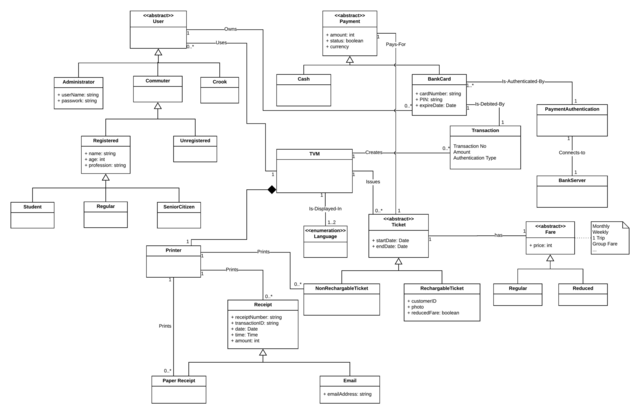
\includegraphics[width=1\textwidth]{domain_model.png}
	\caption{\label{fig:Use Case Model : } Change Language Use Case Model}	
\end{figure}


\newpage
\section{Problem 4}
\subsection{Use Case Model}

\vspace{0.5cm}
\textbf{\large Use Case: Change Language} 
\\ 

\begin{tabular}{ | c | p{2cm} | p{7cm} |}
	
	\hline
	\textbf{Number} & \multicolumn{2}{c|}{1}  \\
	\hline
	\textbf{Name} & \multicolumn{2}{c|}{Change Language}  \\
	\hline
	\textbf{Summary} & \multicolumn{2}{c|}{User wants to change to desired language }  \\
	\hline
	\textbf{Priority} & \multicolumn{2}{c|}{4}  \\
	\hline
	\textbf{Preconditions} & \multicolumn{2}{c|}{N/A}  \\
	\hline
	\textbf{Postconditions} & \multicolumn{2}{c|}{User is able to change to desired language}  \\
	\hline
	\textbf{Primary Actor(s)} & \multicolumn{2}{c|}{TVM Customer}  \\
	\hline
	\textbf{Secondary Actors(s)} & \multicolumn{2}{c|}{TVM and Administrator}  \\
	\hline
	\textbf{Trigger} & \multicolumn{2}{c|}{User has chosen to change language}  \\
	\hline
	\textbf{Main Success Scenarios} & \textbf{Step} & \textbf{Action} \\
	\hline
	  & 1 & User can select the desired language \\ 
	\hline
	  &  2  & The application is displayed in desired language \\
	\hline
	\textbf{Extensions} & \multicolumn{2}{c|}{N/A}  \\
	\hline
	\textbf{Open Issues} &  1  & Language available to be decided by the customer \\
	\hline
	
\end{tabular}

\begin{figure}[!htb]
	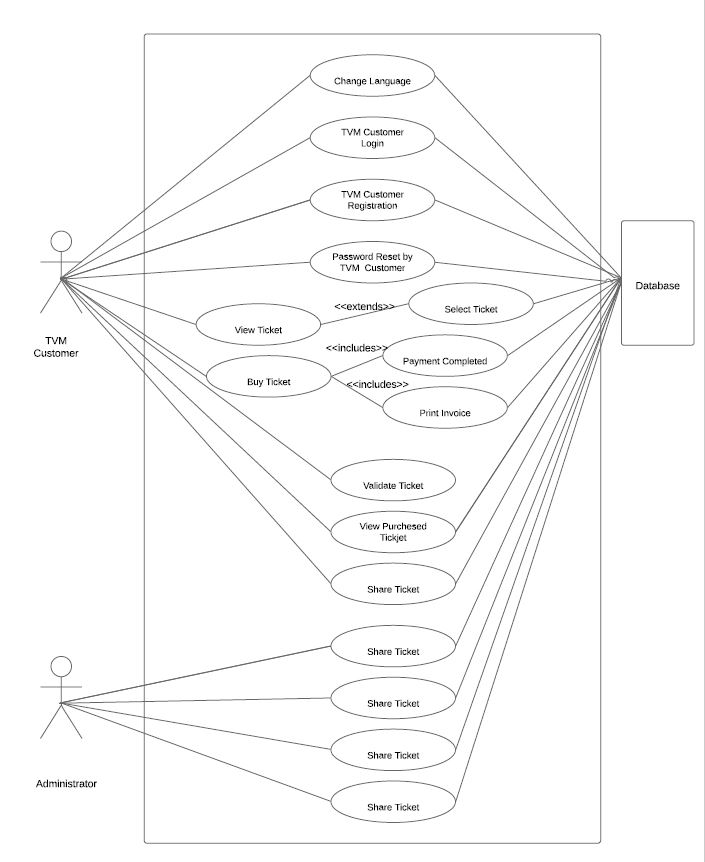
\includegraphics[width=1\textwidth]{Use_Case_Diagrams/ChangeLanguage.JPG}
	\caption{\label{fig:Use Case Model : } Change Language Use Case Model}	
\end{figure} 

\vspace{0.5cm}
\textbf{\large Use Case: View Ticket Plans}
\\

\begin{tabular}{ | c | p{2cm} | p{7cm} |}
	
	\hline
	\textbf{Number} & \multicolumn{2}{c|}{2}  \\
	\hline
	\textbf{Name} & \multicolumn{2}{c|}{View Ticket Plans}  \\
	\hline
	\textbf{Summary} & \multicolumn{2}{c|}{User has viewed different ticket plans}  \\
	\hline
	\textbf{Priority} & \multicolumn{2}{c|}{1}  \\
	\hline
	\textbf{Preconditions} & \multicolumn{2}{c|}{N/A}  \\
	\hline
	\textbf{Postconditions} & \multicolumn{2}{c|}{User has viewed different ticket plans}  \\
	\hline
	\textbf{Primary Actor(s)} & \multicolumn{2}{c|}{TVM Customer}  \\
	\hline
	\textbf{Secondary Actors(s)} & \multicolumn{2}{c|}{Data Store}  \\
	\hline
	\textbf{Trigger} & \multicolumn{2}{c|}{User has chosen to view ticket plans}  \\
	\hline
	\textbf{Main Success Scenarios} & \textbf{Step} & \textbf{Action} \\
	\hline
	& 1 & User selects the language \\ 
	\hline
	&  2  & System asks the ticket type \\
	\hline
	&  3  & User selects the ticket type \\
	\hline
	&  2  & System displays ticket plans \\
	\hline
	\textbf{Extensions} & \multicolumn{2}{c|}{N/A}  \\
	\hline
	\textbf{Open Issues} &    & NA \\
	\hline
	
\end{tabular}

\begin{figure}[!htb]
	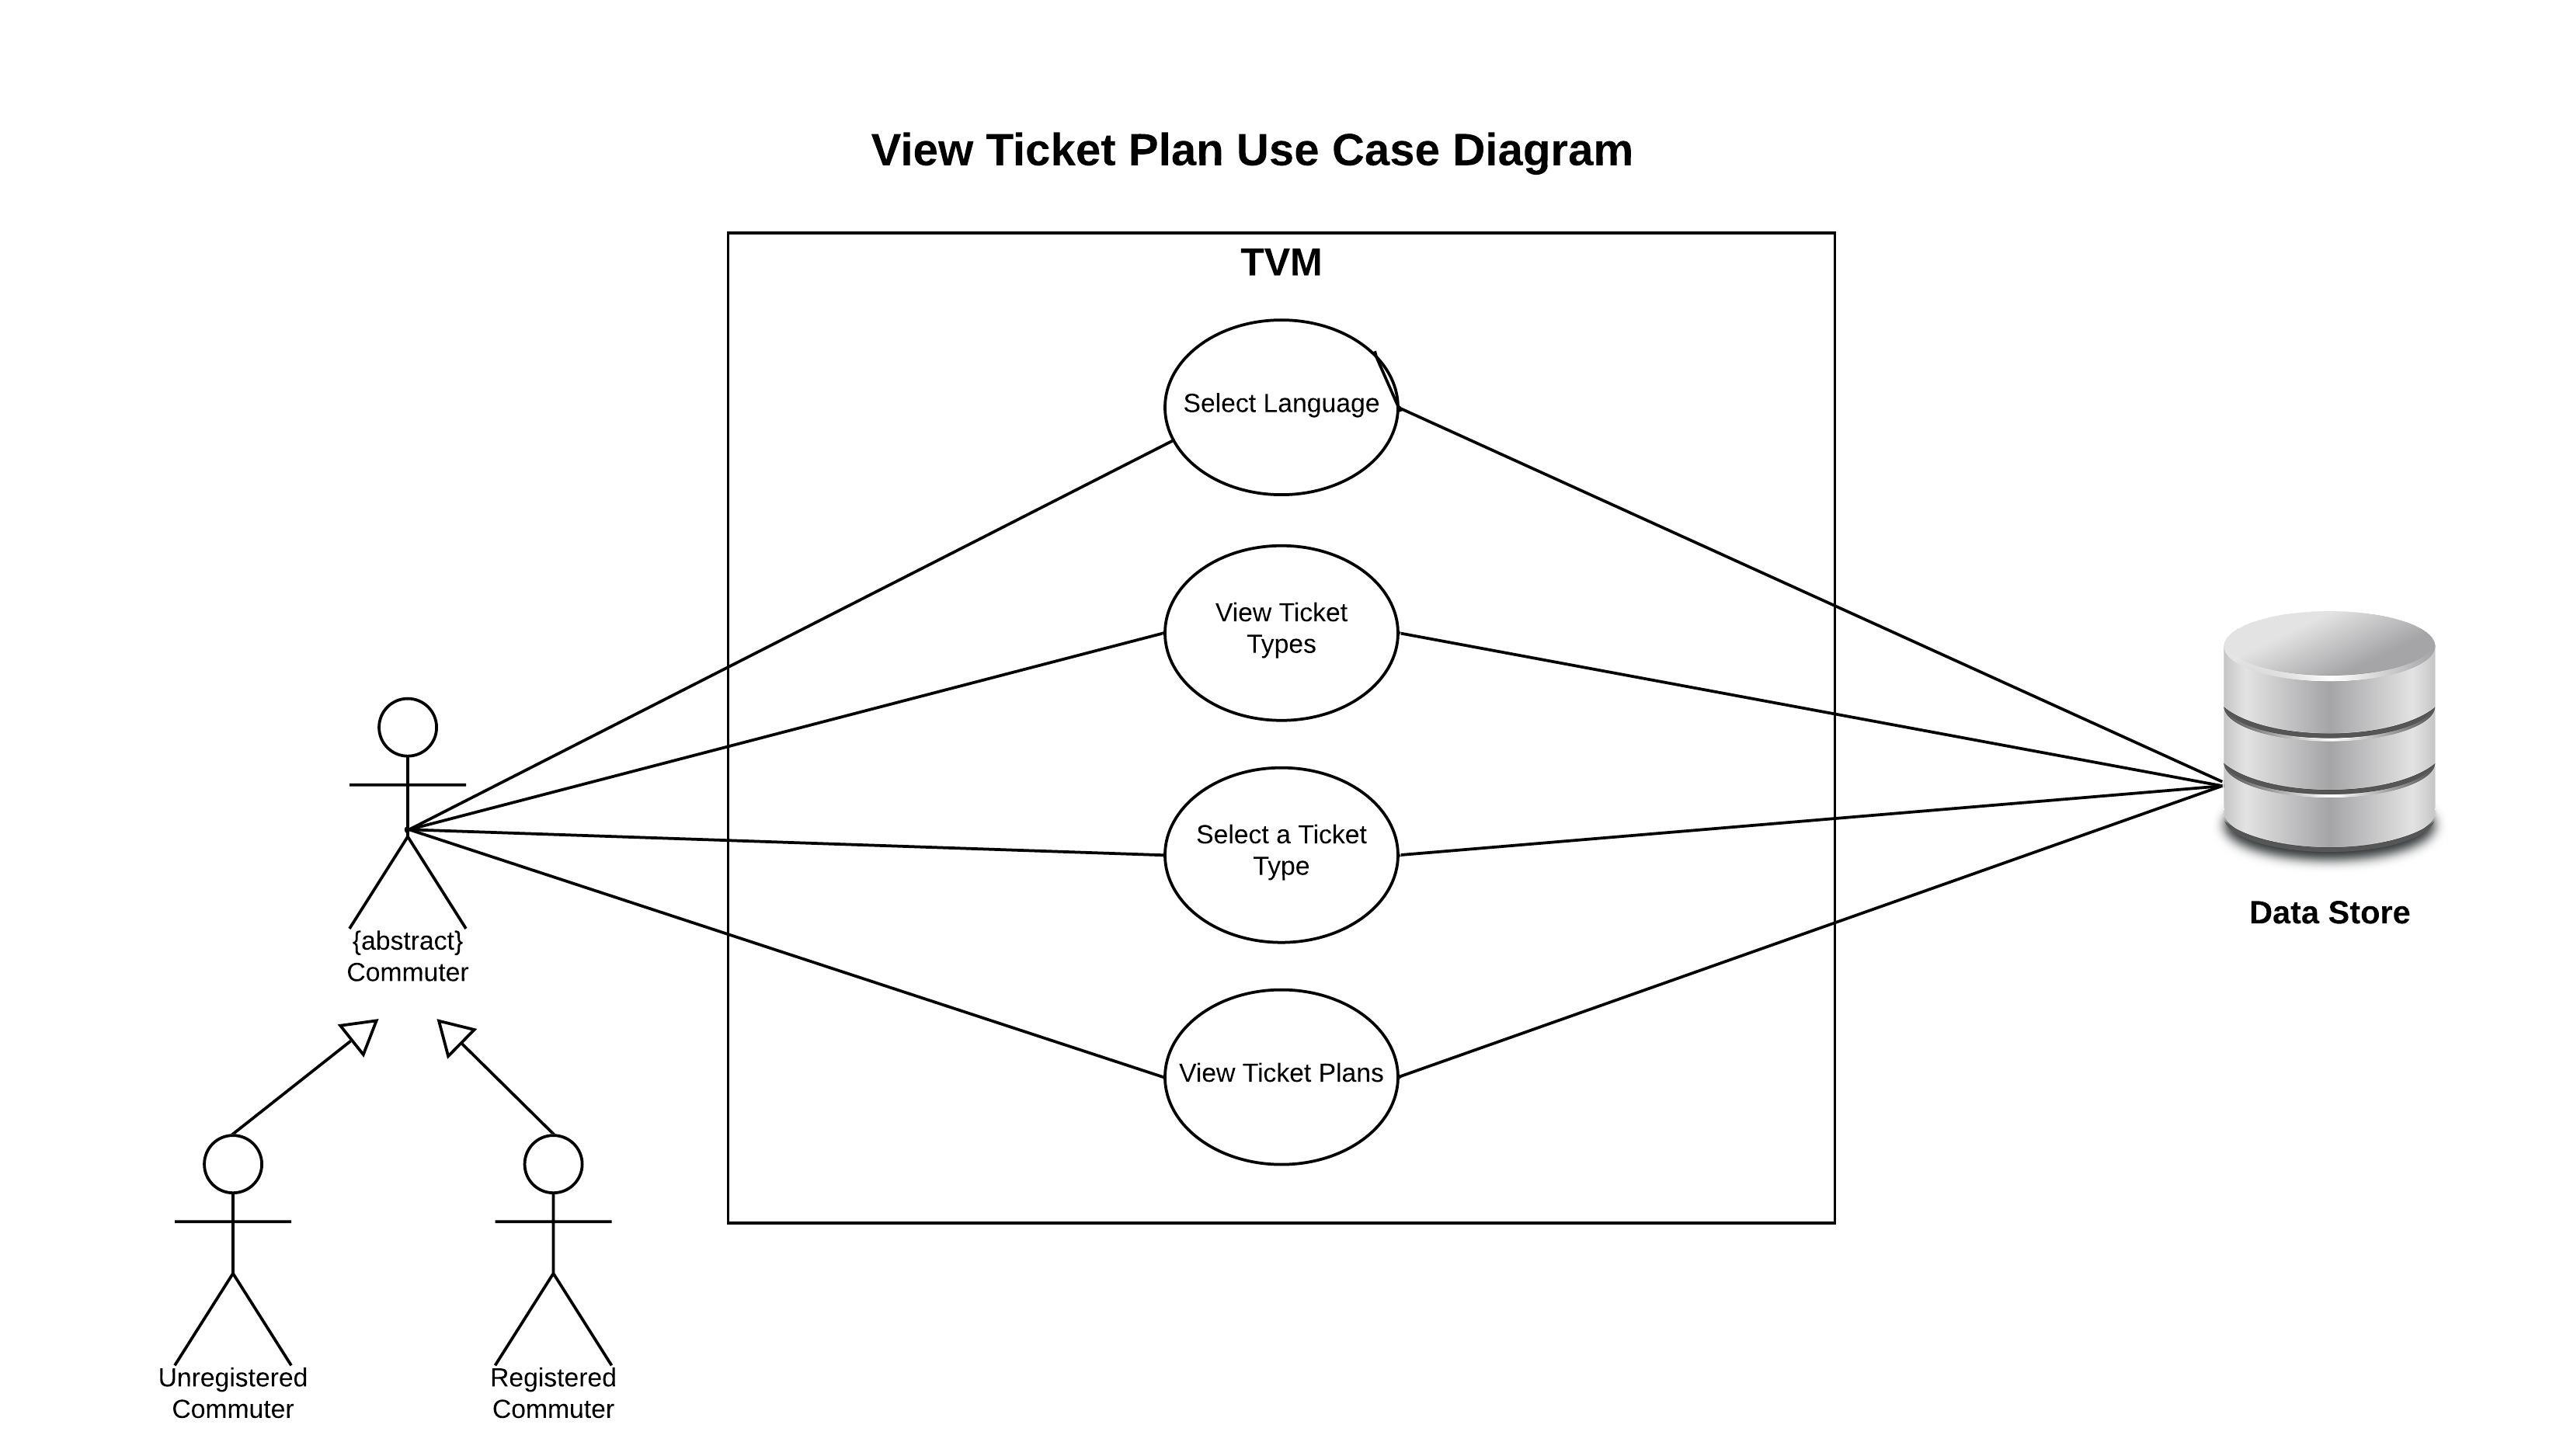
\includegraphics[width=1\textwidth]{Use_Case_Diagrams/ViewTicketPlan.jpeg}
	\caption{\label{fig:Use Case Model : } View Ticket Plans}	
\end{figure}


\vspace{0.5cm}
\textbf{\large Use Case: Buy Tickets}
\\

\begin{tabular}{ | c | p{2cm} | p{7cm} |}
	
	\hline
	\textbf{Number} & \multicolumn{2}{c|}{3}  \\
	\hline
	\textbf{Name} & \multicolumn{2}{c|}{Buy Ticket}  \\
	\hline
	\textbf{Summary} & \multicolumn{2}{c|}{Customer buy a ticket using TVM}  \\
	\hline
	\textbf{Priority} & \multicolumn{2}{c|}{1}  \\
	\hline
	\textbf{Preconditions} & \multicolumn{2}{c|}{Customer has access to a valid payment method}  \\
	\hline
	\textbf{Postconditions} & \multicolumn{2}{c|}{Customer has received the ticket and the receipt}  \\
	\hline
	\textbf{Primary Actor(s)} & \multicolumn{2}{c|}{TVM Customer}  \\
	\hline
	\textbf{Secondary Actors(s)} & \multicolumn{2}{c|}{Payment Authentication, Bank Server, Data Store}  \\
	\hline
	\textbf{Trigger} & \multicolumn{2}{c|}{Customer has chosen to buy a ticket}  \\
	\hline
	\textbf{Main Success Scenarios} & \textbf{Step} & \textbf{Action} \\
	\hline
	& 1 & Customer selects the language \\ 
	\hline
	&  2  & System displays ticket plans \\
	\hline
	&  3  & Customer chooses a ticket plan \\
	\hline
	&  4  & System asks for payment method \\
	\hline
	&  5  & Customer selects a payment method \\
	\hline
	&  6  & Customer makes a payment \\
	\hline
	&  7  & System asks for type of receipt \\
	\hline
	&  8  & Customer selects the type of receipt \\
	\hline
	&  9  & System prints receipt and ticket \\
	\hline
	&  10  & Customer removes receipt and ticket \\
	\hline
	&  11  & System displays welcome message \\
	\hline
	\textbf{Extensions} & \textbf{Step} & \textbf{Branching Action} \\
	\hline
	&  6a  & The payment is not successful \\
	\hline
	&  6b  & System displays message that payment is not successful \\
	\hline
	&  6c  & System exits and displays welcome message \\
	\hline
	\textbf{Open Issues} &    & NA \\
	\hline
	
\end{tabular}

\begin{figure}[!htb]
	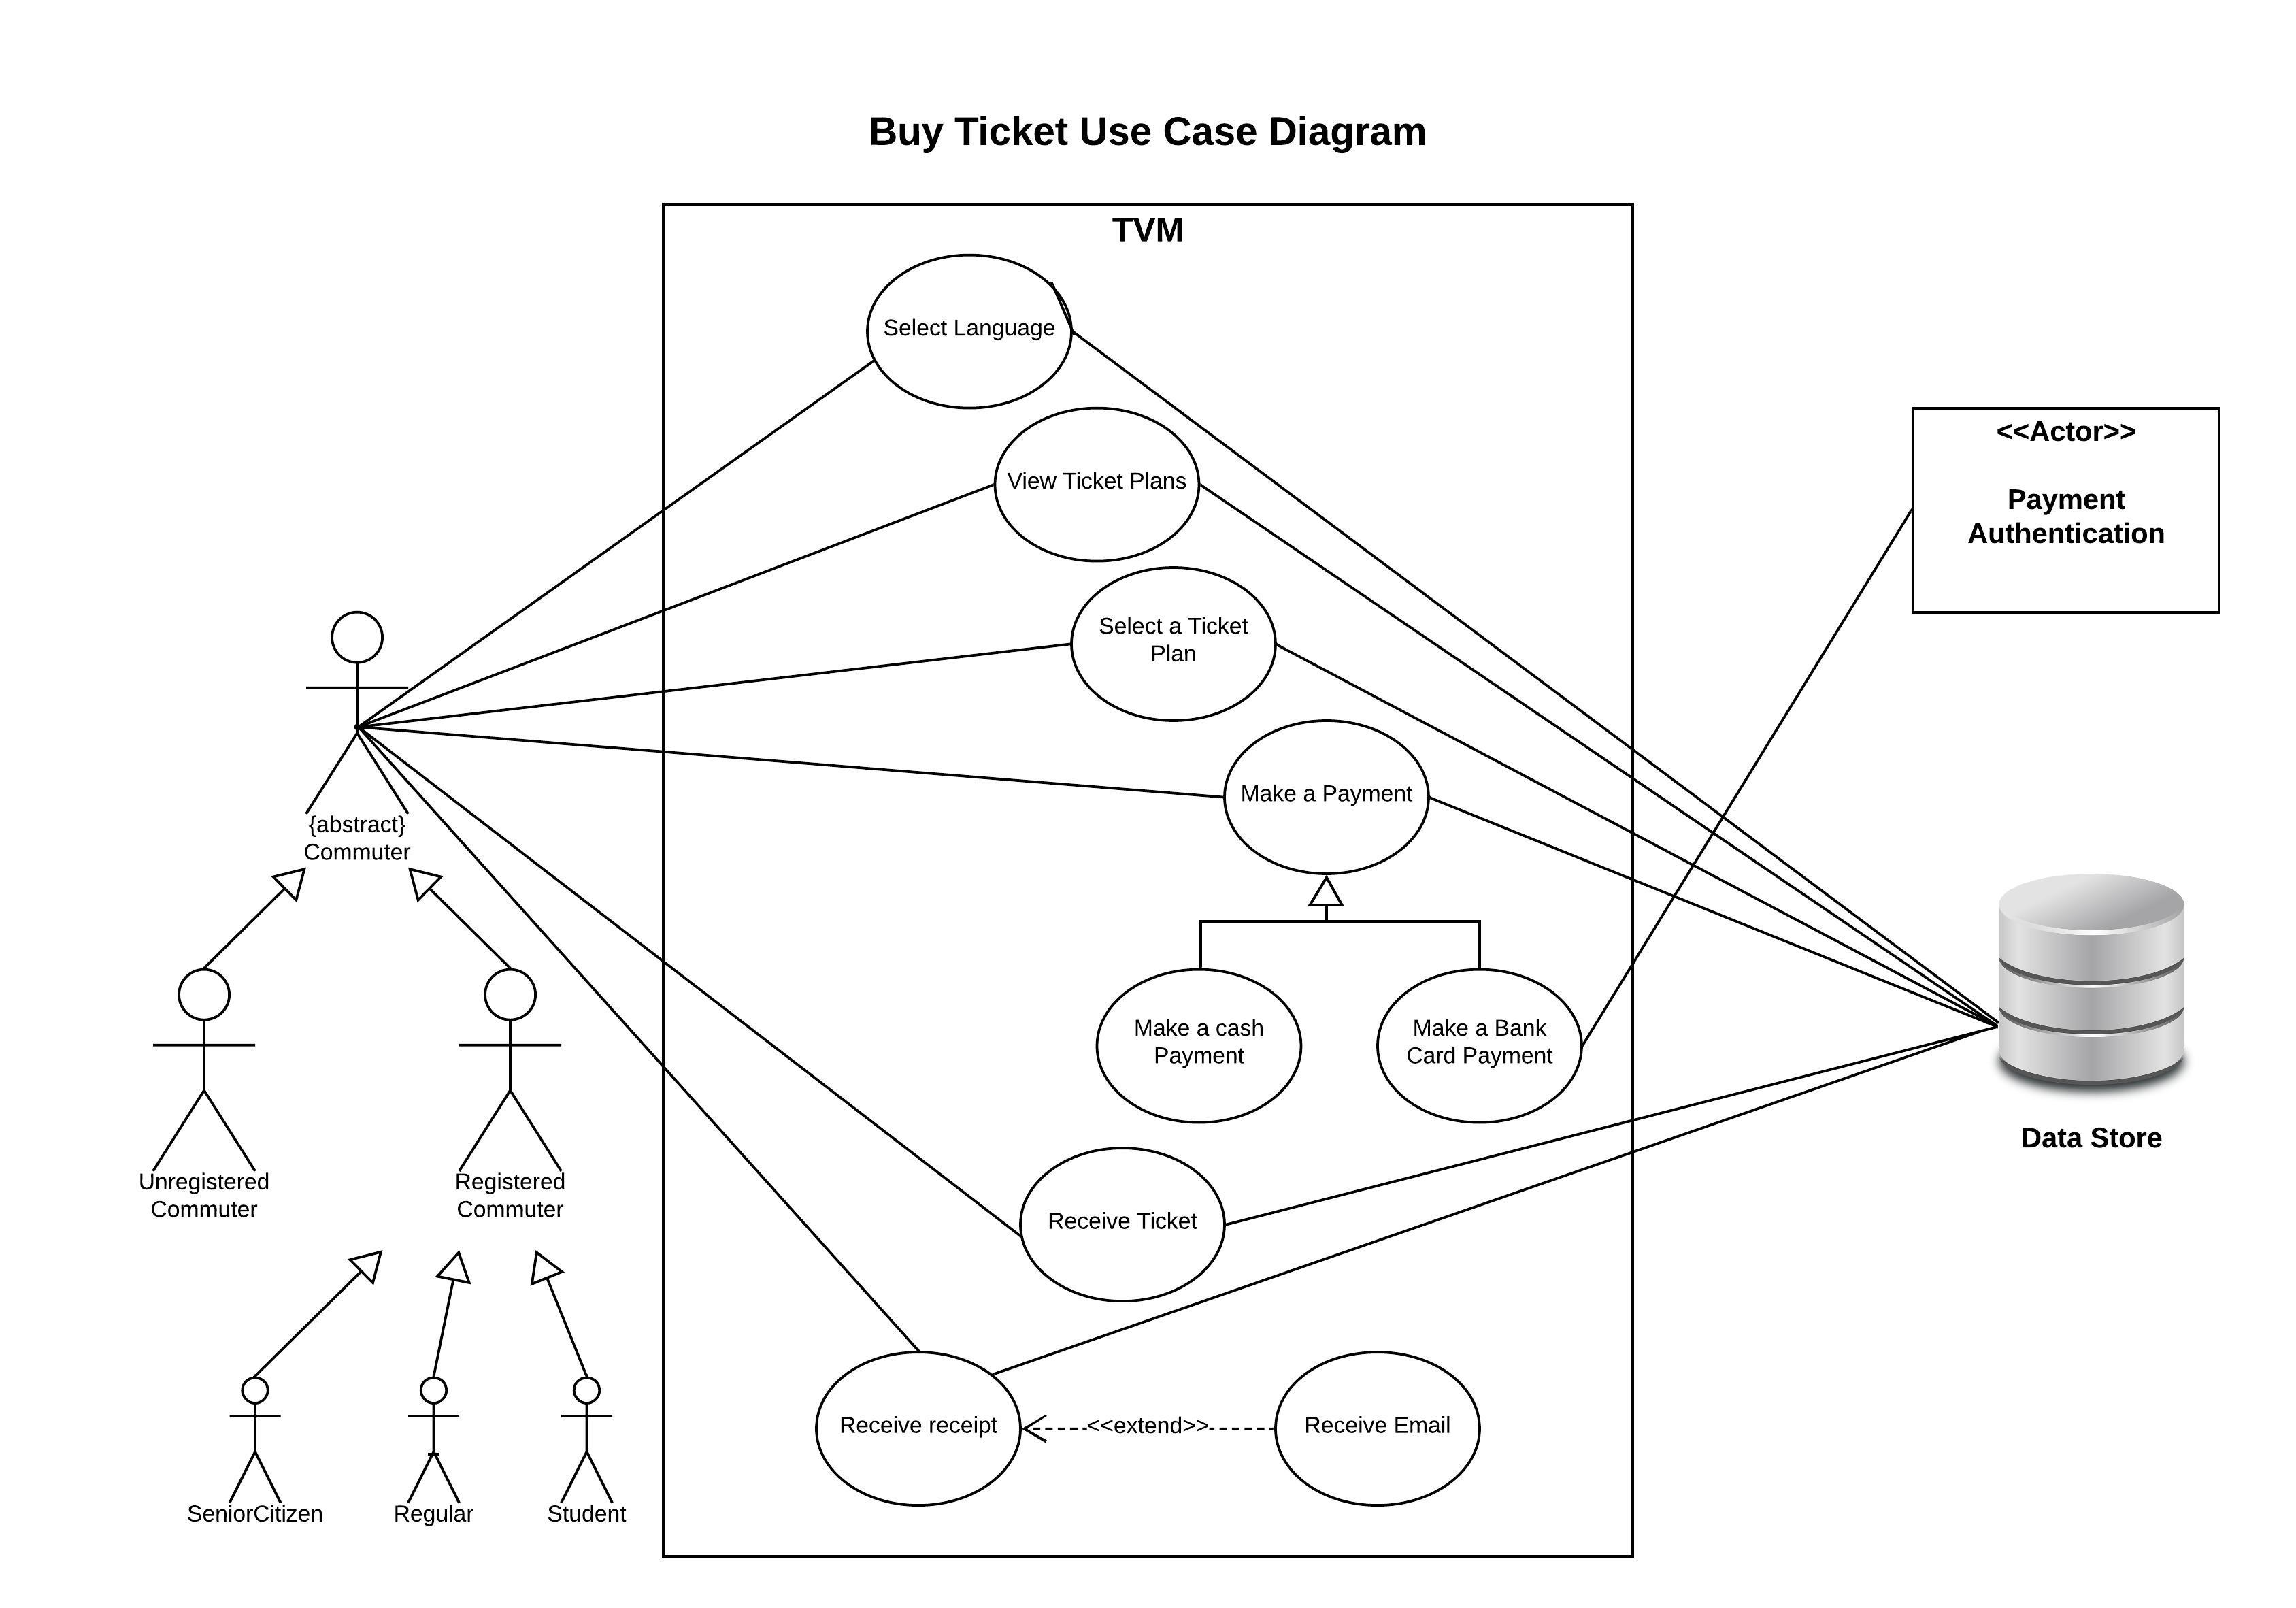
\includegraphics[width=1\textwidth]{Use_Case_Diagrams/BuyTicket.jpeg}
	\caption{\label{fig:Use Case Model : } Buy Ticket}	
\end{figure}


\vspace{0.5cm}
\textbf{\large Use Case: Make a payment}
\\

\begin{tabular}{ | c | p{2cm} | p{7cm} |}
	
	\hline
	\textbf{Number} & \multicolumn{2}{c|}{4}  \\
	\hline
	\textbf{Name} & \multicolumn{2}{c|}{Make a Credit Card Payment, Make a cash Payment}  \\
	\hline
	\textbf{Summary} & \multicolumn{2}{c|}{Customer make payment by card or cash using TVM}  \\
	\hline
	\textbf{Priority} & \multicolumn{2}{c|}{1}  \\
	\hline
	\textbf{Preconditions} & \multicolumn{2}{c|}{User has a valid credit card, valid currency}  \\
	\hline
	\textbf{Postconditions} & \multicolumn{2}{c|}{Transaction successful, user should get the ticket.}  \\
	\hline
	\textbf{Primary Actor(s)} & \multicolumn{2}{c|}{TVM Customer / Bank Card Reader / Cash Receiver.}  \\
	\hline
	\textbf{Secondary Actors(s)} & \multicolumn{2}{c|}{Payment Gateway.}  \\
	\hline
	\textbf{Trigger} & \multicolumn{2}{c|}{User has chosen to buy a metro ticket}  \\
	\hline
	\textbf{Main Success Scenarios} & \textbf{Step} & \textbf{Action} \\
	\hline
	& 1 & System displays ticket types \\ 
	\hline
	&  2  & User chooses the type of ticket \\
	\hline
	&  3  & System asks for payment method \\
	\hline
	&  4  & User select pay by cash or card \\
	\hline
	&  5  & System asks user to insert his card or cash (to cash receiver). \\
	\hline
	&  6  & User insert his cash or card. \\
	\hline
	&  7  & System asks user to enter the PIN (in case of card payment) \\
	\hline
	&  8  & User enter the PIN \\
	\hline
	&  9  & System connects to the payment gateway and authentication the user details. \\
	\hline
	&  10  & System create a transaction and records the transaction. \\
	\hline
	&  11  & System asks how user wants to receive the receipt \\
	\hline
	&  12  & User select paper receipt \\
	\hline
	&  13  & System prints and dispenses receipt and ticket \\
	\hline
	&  14  & User takes out receipt and ticket. \\
	\hline
	&  15  & System displays a message to remove the credit card \\
	\hline
	&  16  & User removes card \\
	\hline
	&  17  & System displays welcome message. \\
	\hline
	
	\textbf{Extensions} & \textbf{Step} & \textbf{Branching Action} \\
	\hline
	&  6a  & User insert card into card reader. \\
	\hline
	&  6b  & User insert cash into the cash receiver. \\
	\hline
	&  7a  & No pin asked in case of cash payment. \\
	\hline
	&  9a  & System authenticated the cash denominations in case of cash payment. \\
	\hline
	&  11a  & If payment is not successful user will not receive the print receipt message. \\
	\hline
	&  15a  & No message displayed in case of cash payment. \\
	\hline
	\textbf{Open Issues} &    & NA \\
	\hline
	
\end{tabular}


%\begin{figure}[!htb]
%	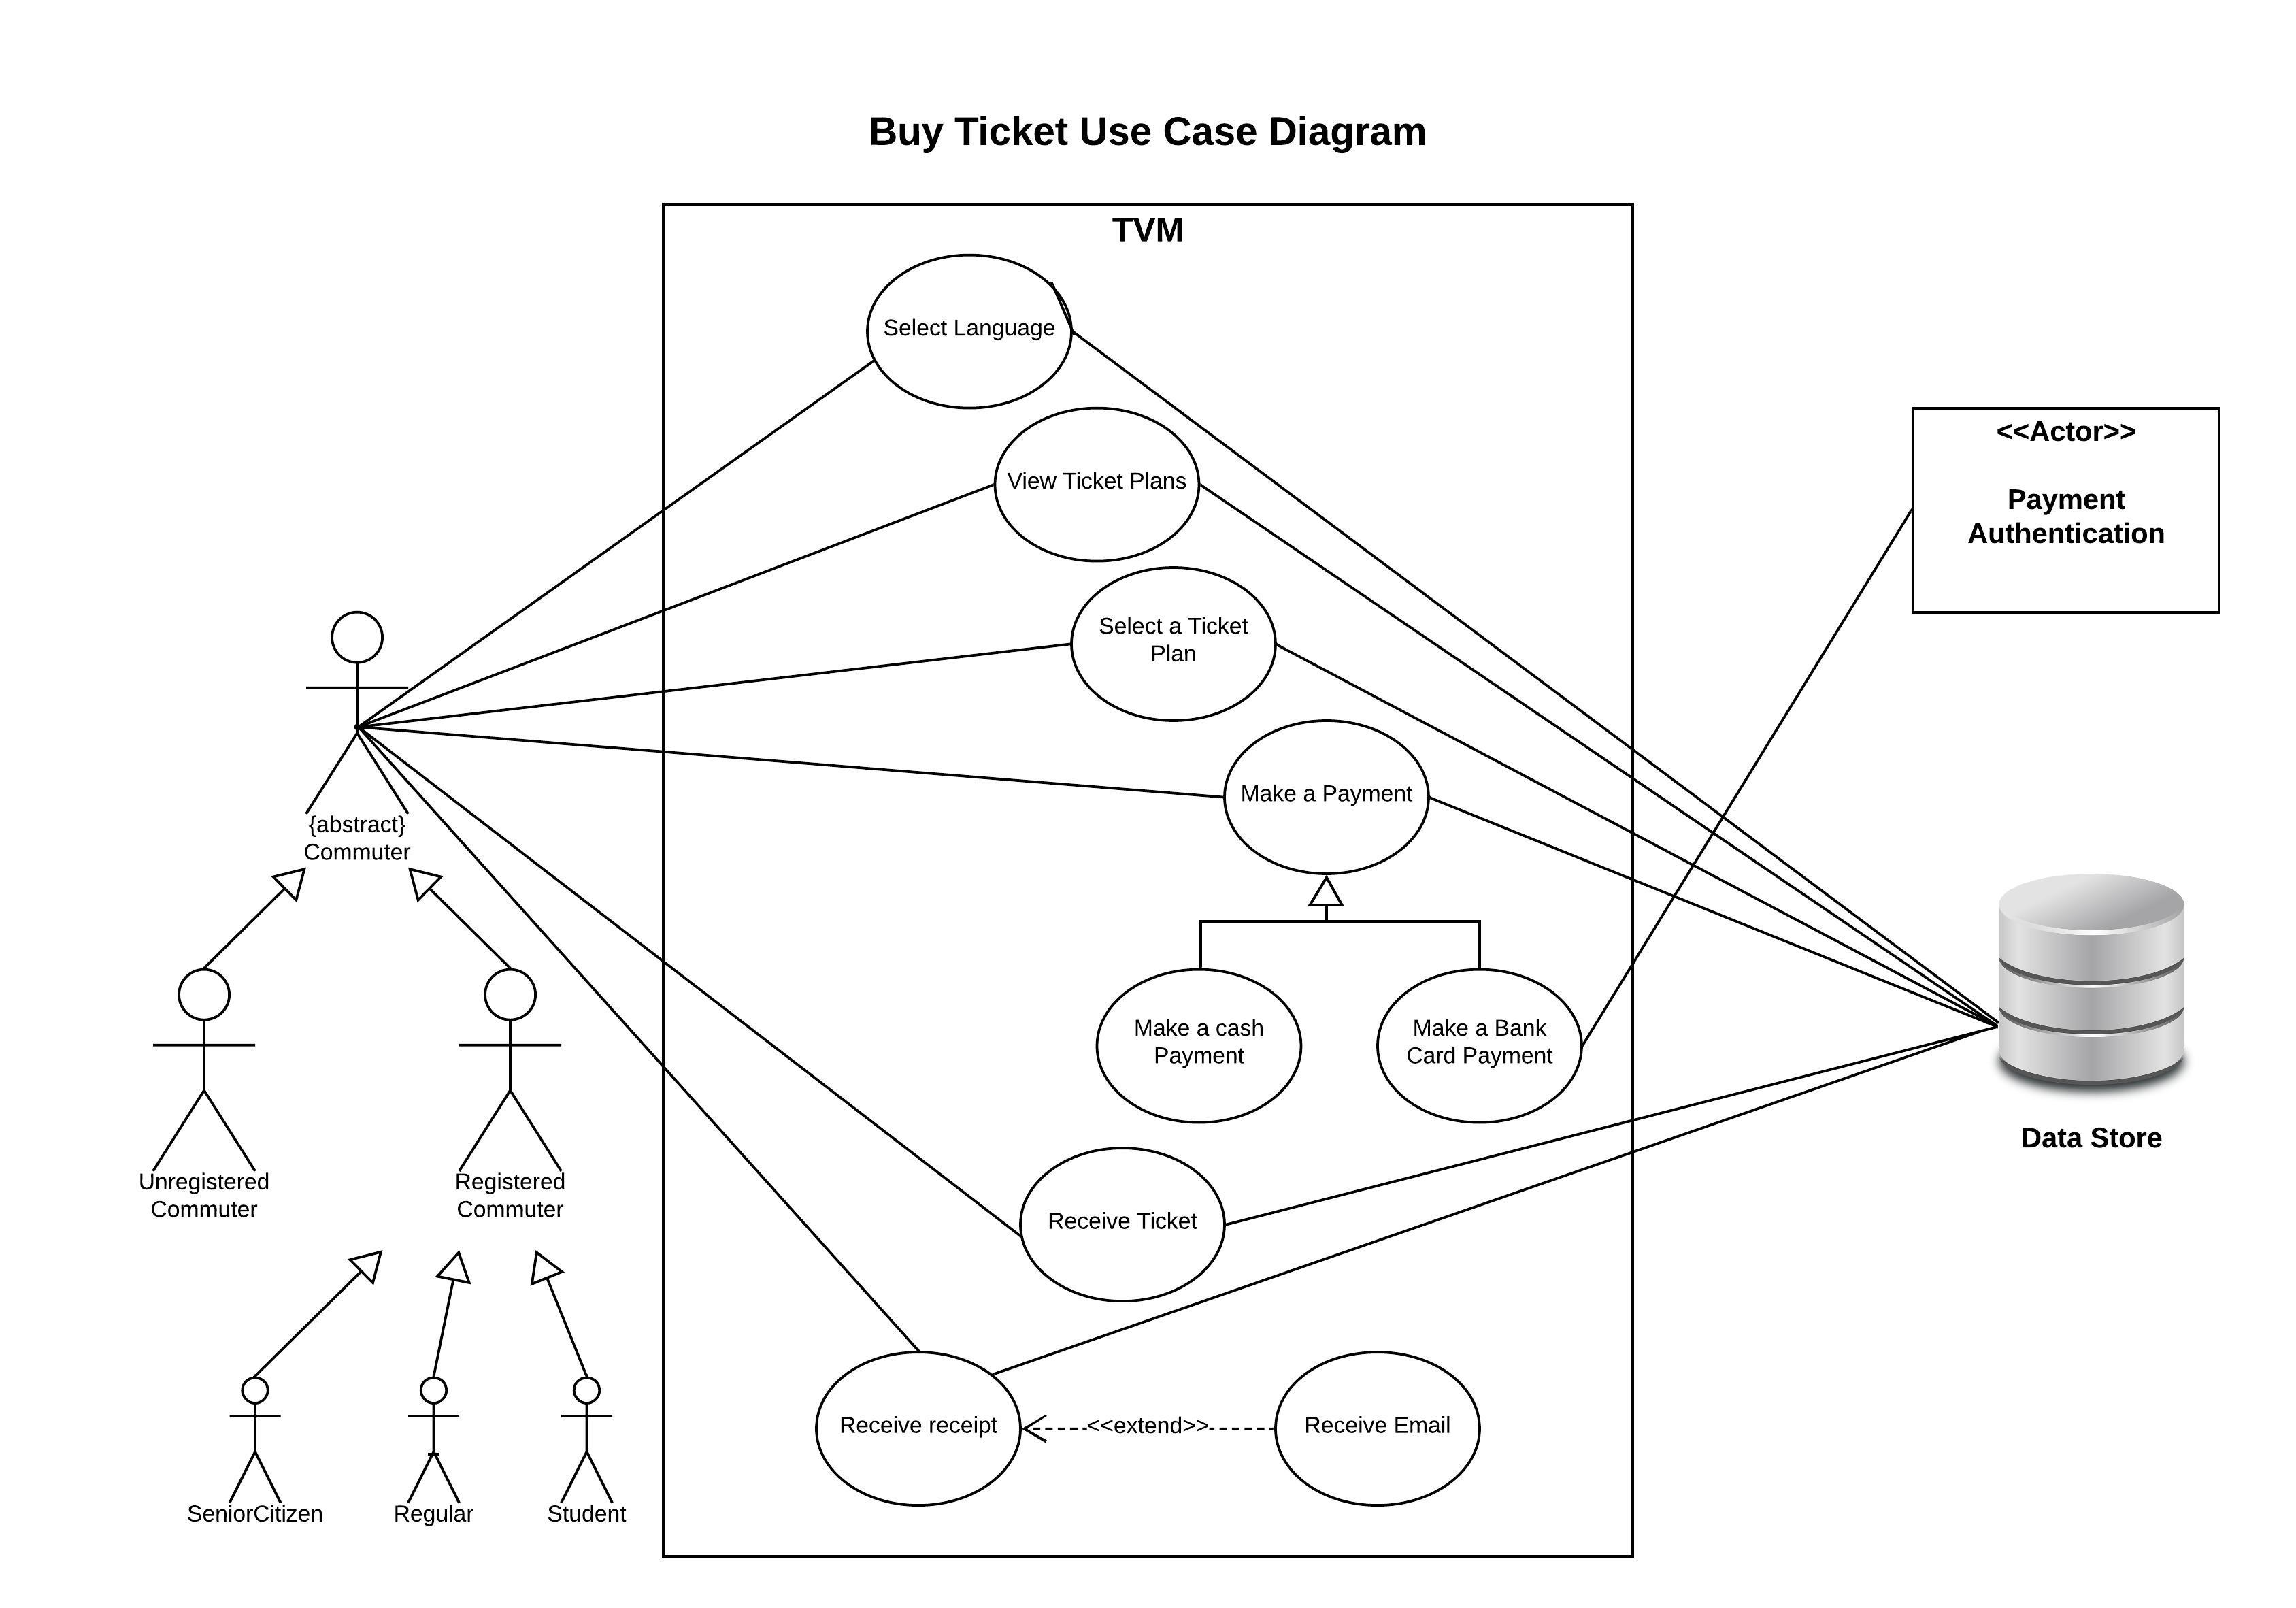
\includegraphics[width=1\textwidth]{Use_Case_Diagrams/BuyTicket.jpeg}
%	\caption{\label{fig:Use Case Model : } Buy Ticket}	
%\end{figure}


\vspace{0.5cm}
\textbf{\large Use Case: Reload Rechargeable Card}
\\

\begin{tabular}{ | c | p{2cm} | p{7cm} |}
	
	\hline
	\textbf{Number} & \multicolumn{2}{c|}{5}  \\
	\hline
	\textbf{Name} & \multicolumn{2}{c|}{Reload Rechargeable Card}  \\
	\hline
	\textbf{Summary} & \multicolumn{2}{c|}{Customer reloads the rechargeable card using TVM}  \\
	\hline
	\textbf{Priority} & \multicolumn{2}{c|}{5}  \\
	\hline
	\textbf{Preconditions} & \multicolumn{2}{c|}{User has a Rechargeable card}  \\
	\hline
	\textbf{Postconditions} & \multicolumn{2}{c|}{User has recharged the card and received a receipt}  \\
	\hline
	\textbf{Primary Actor(s)} & \multicolumn{2}{c|}{TVM Customer}  \\
	\hline
	\textbf{Secondary Actors(s)} & \multicolumn{2}{c|}{Data Store}  \\
	\hline
	\textbf{Trigger} & \multicolumn{2}{c|}{User has chosen to reload the card}  \\
	\hline
	\textbf{Main Success Scenarios} & \textbf{Step} & \textbf{Action} \\
	\hline
	& 1 & User inserts the rechargeable card in the machine \\ 
	\hline
	&  2  & User selects the language \\
	\hline
	&  3  & User select the option to recharge the card \\
	\hline
	&  4  & System displays different recharge plans \\
	\hline
	&  5  & User chooses the recharge plan \\
	\hline
	&  6  & System asks for the payment method \\
	\hline
	&  7  & User choses the way of payment \\
	\hline
	&  8  & User done with the payment \\
	\hline
	&  9  & System displays the message to retrieve the rechargeable card \\
	\hline
	&  10  & User removes the card. \\
	\hline
	&  11  & System asks the user if he wants to print receipt \\
	\hline
	&  12  & User select the option from Yes or No \\
	\hline
	&  13  & System prints and dispenses receipt \\
	\hline
	&  14  & System displays welcome message \\
	\hline
	
	\textbf{Extensions} & \textbf{Step} & \textbf{Branching Action} \\
	\hline
	\textbf{Open Issues} &    & NA \\
	\hline
	
\end{tabular}


\begin{figure}[!htbp]
	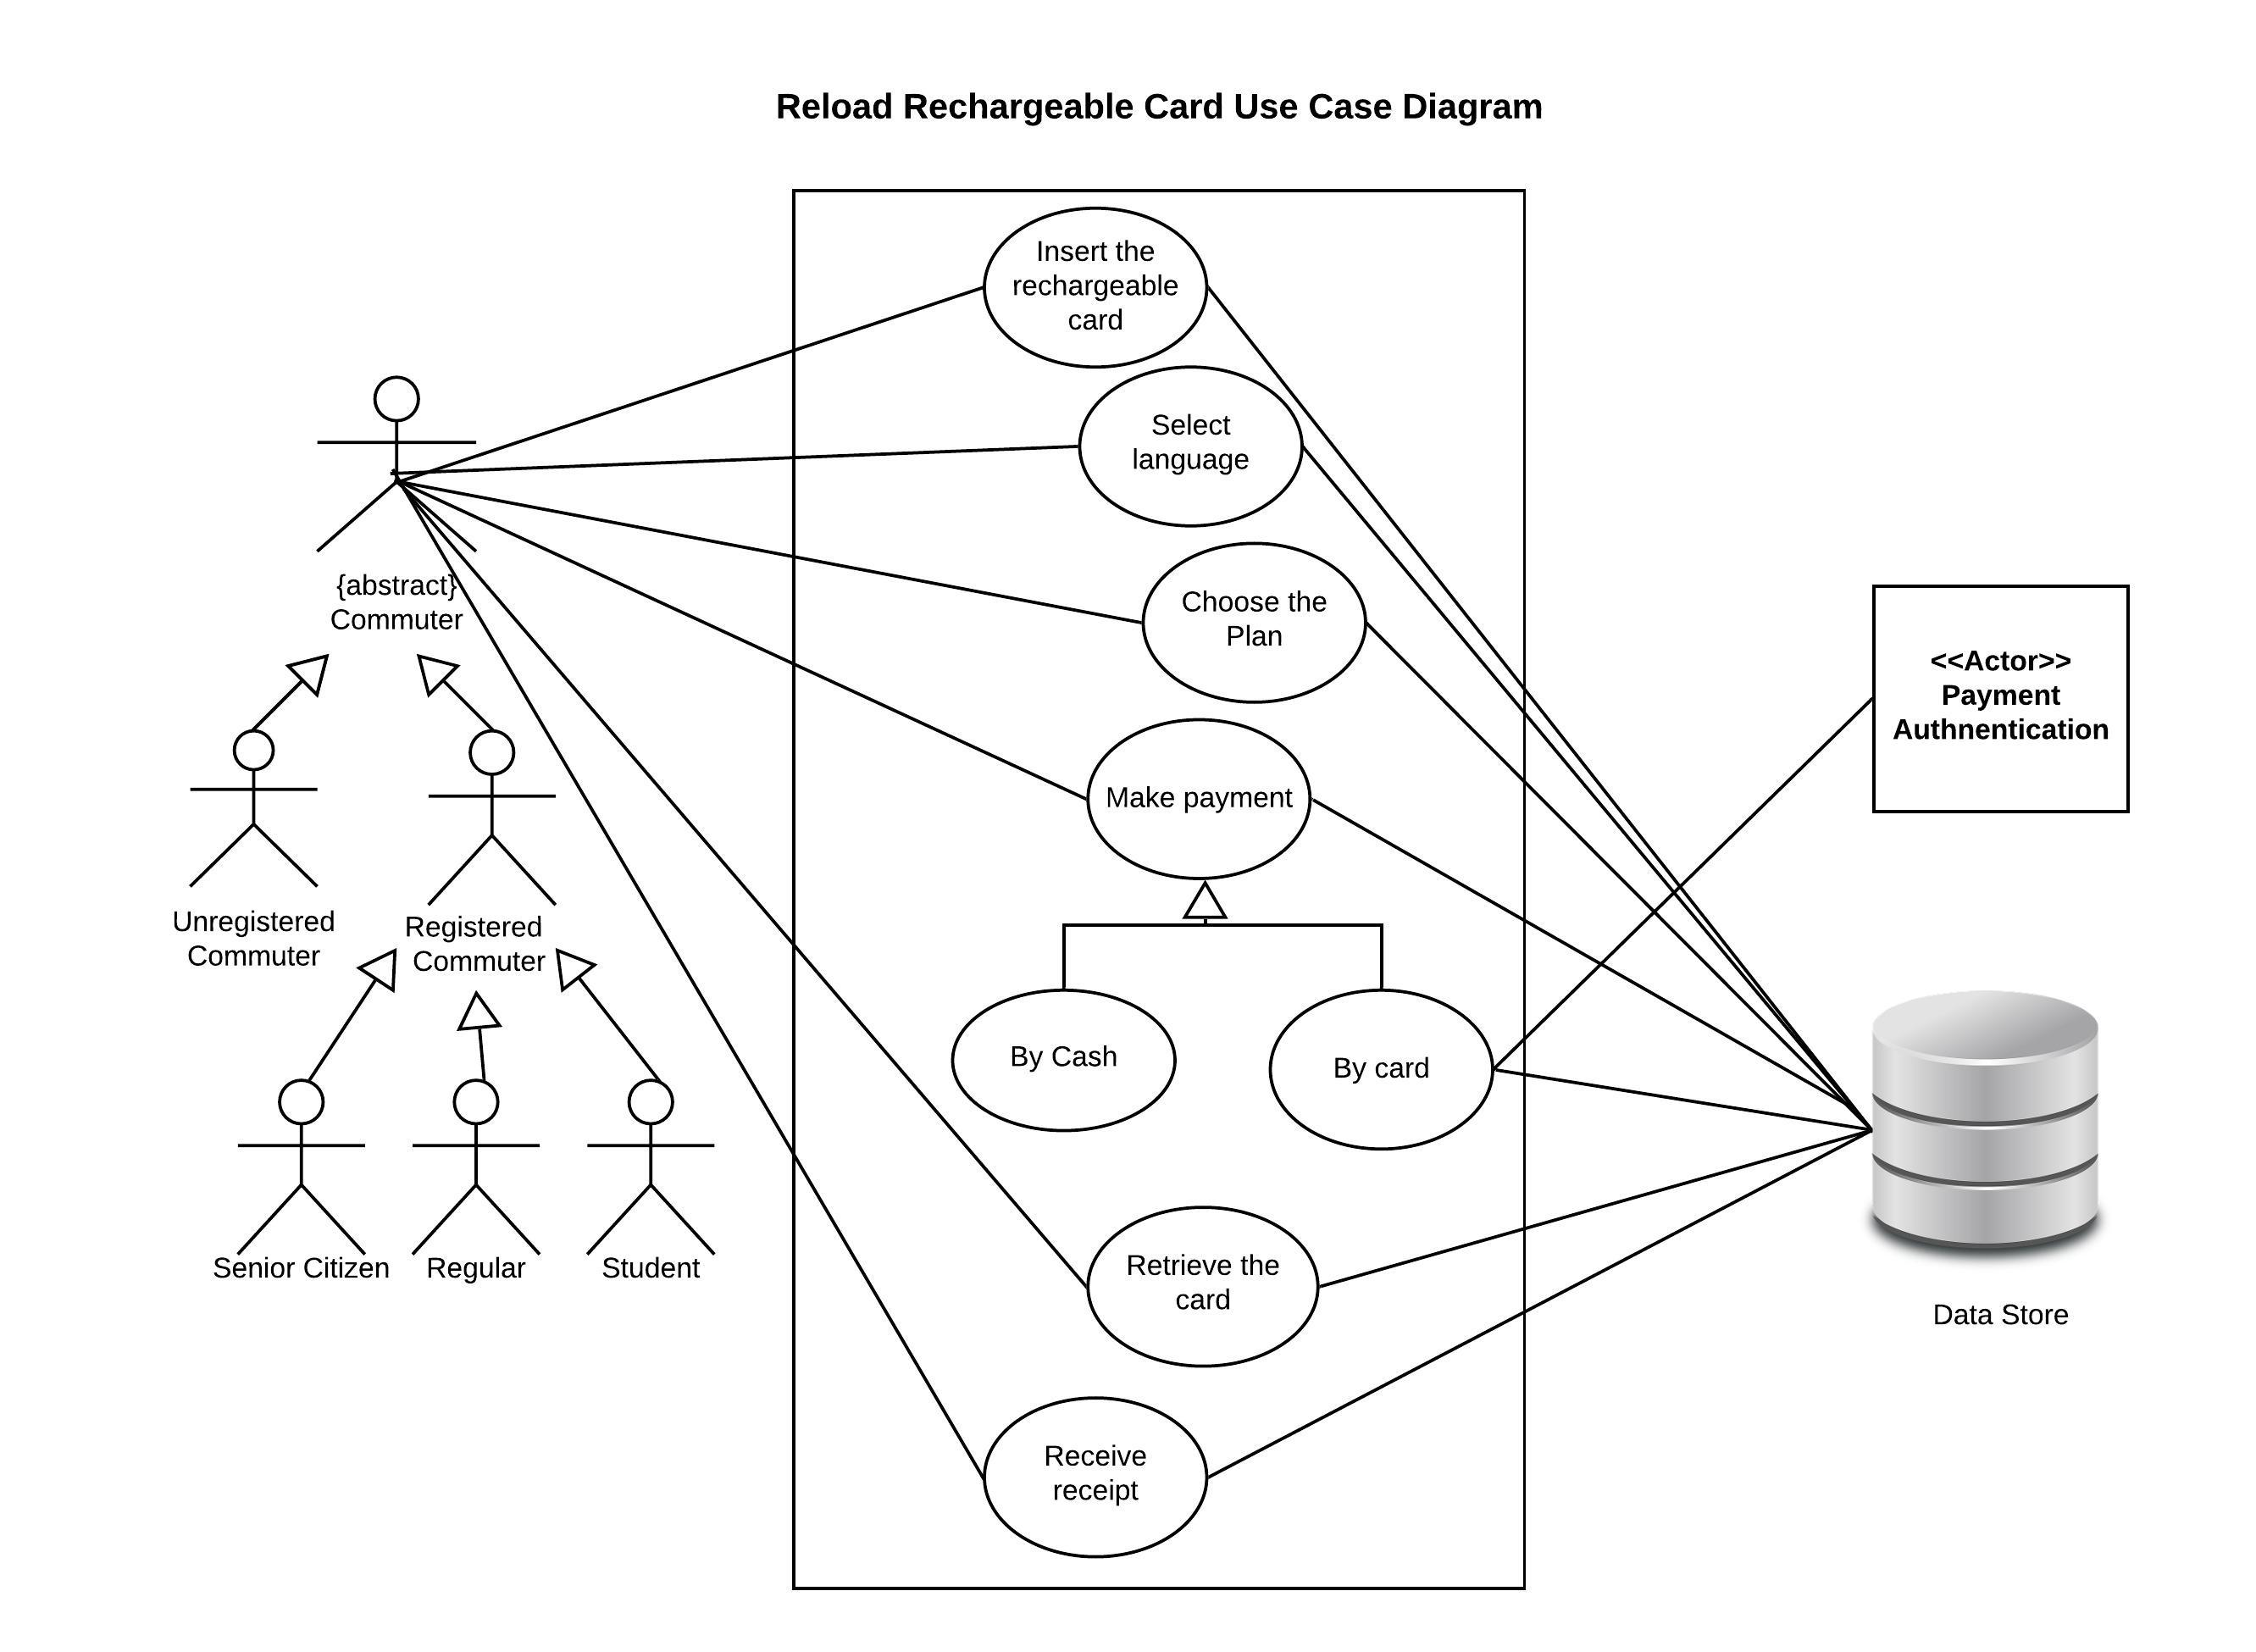
\includegraphics[width=1\textwidth]{Use_Case_Diagrams/ReloadCard.jpeg}
	\caption{\label{fig:Use Case Model : } Reload Rechargeable Card}	
\end{figure}



\vspace{0.5cm}
\textbf{\large Use Case: Update Ticket Specification}
\\

\begin{tabular}{ | c | p{2cm} | p{7cm} |}
	
	\hline
	\textbf{Number} & \multicolumn{2}{c|}{6}  \\
	\hline
	\textbf{Name} & \multicolumn{2}{c|}{Update Ticket Specification}  \\
	\hline
	\textbf{Summary} & \multicolumn{2}{c|}{Administrator to update an existing ticket specifications}  \\
	\hline
	\textbf{Priority} & \multicolumn{2}{c|}{2}  \\
	\hline
	\textbf{Preconditions} & \multicolumn{2}{c|}{Administrator should have a valid account}  \\
			  &  \multicolumn{2	}{c|}{Administrator should be logged into the application} \\
	\hline
	\textbf{Postconditions} & \multicolumn{2}{c|}{Administrator is able to edit an exiting ticket plan.}  \\
	\hline
	\textbf{Primary Actor(s)} & \multicolumn{2}{c|}{TVM Administrator}  \\
	\hline
	\textbf{Secondary Actors(s)} & \multicolumn{2}{c|}{TVM and Customer}  \\
	\hline
	\textbf{Trigger} & \multicolumn{2}{c|}{The Administrator has selected to update}  \\
     	&  \multicolumn{2	}{c|}{ ticket specifications on the system.}} \\
	\hline
	\textbf{Main Success Scenarios} & \textbf{Step} & \textbf{Action} \\
	\hline
	& 1 & Admin selects the tickets to be modified. \\ 
	\hline
	&  2  & Admin change the ticket specification. \\
	\hline
	&  3  & Admin saves the new ticket specifications. \\
	\hline
	&  4  & Admin updates the system with updated ticket plans. \\
	\hline
	
	\textbf{Extensions} & \textbf{Step} & \textbf{Branching Action} \\
	\hline
	&  3a  & Admin does not have the admin access to the system.  \\
	\hline
	&  4a  &  The system gives an error. \\
	\hline
	\textbf{Open Issues} &    & NA \\
	\hline
	
\end{tabular}


%\begin{figure}[!htbp]
%	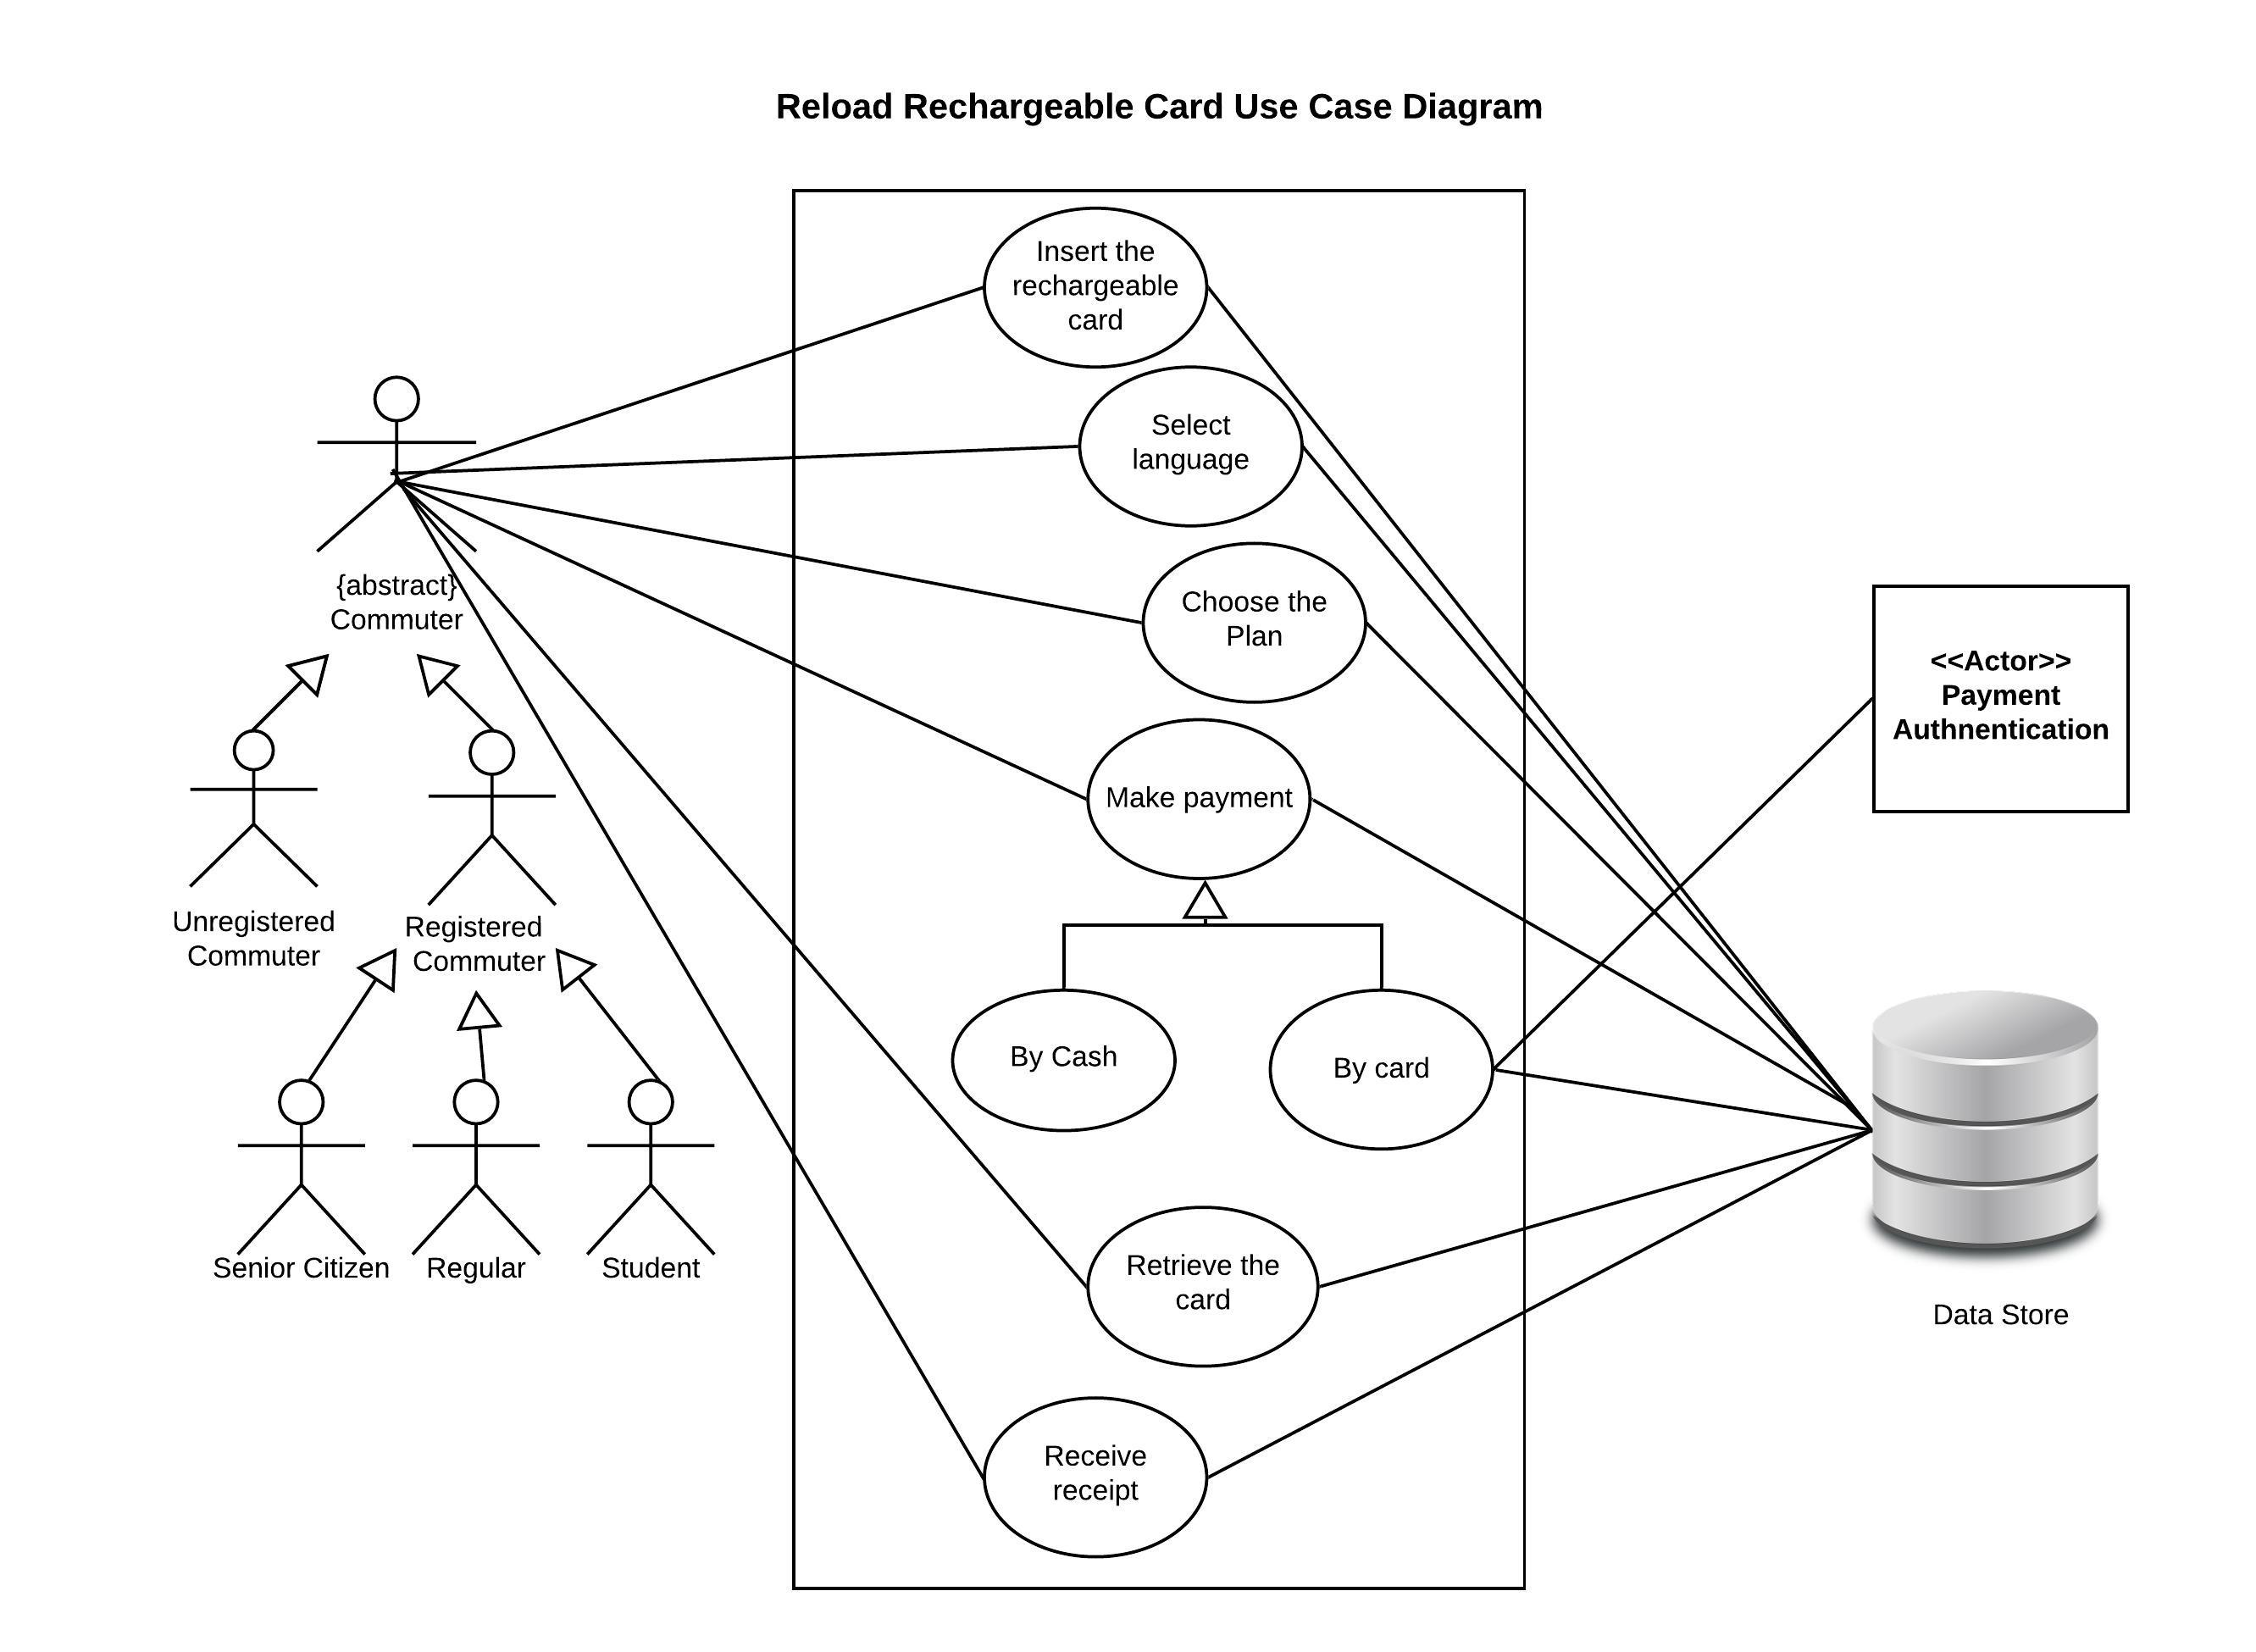
\includegraphics[width=1\textwidth]{Use_Case_Diagrams/ReloadCard.jpeg}
%	\caption{\label{fig:Use Case Model : } Reload Rechargeable Card}	
%\end{figure}


\vspace{0.5cm}
\textbf{\large Use Case: Customer Registration}
\\

\begin{tabular}{ | c | p{2cm} | p{7cm} |}
	
	\hline
	\textbf{Number} & \multicolumn{2}{c|}{7}  \\
	\hline
	\textbf{Name} & \multicolumn{2}{c|}{Customer Registration}  \\
	\hline
	\textbf{Summary} & \multicolumn{2}{c|}{Customer register with his personal information to get the card}  \\
	\hline
	\textbf{Priority} & \multicolumn{2}{c|}{2}  \\
	\hline
	\textbf{Preconditions} & \multicolumn{2}{c|}{N/A}  \\
	\hline
	\textbf{Postconditions} & \multicolumn{2}{c|}{User is registered}  \\
	\hline
	\textbf{Primary Actor(s)} & \multicolumn{2}{c|}{TVM Customer}  \\
	\hline
	\textbf{Secondary Actors(s)} & \multicolumn{2}{c|}{Data Store}  \\
	\hline
	\textbf{Trigger} & \multicolumn{2}{c|}{User has chosen to register himself for the STM} \\
	\hline
	\textbf{Main Success Scenarios} & \textbf{Step} & \textbf{Action} \\
	\hline
	& 1 & User selects the register option \\ 
	\hline
	&  2  & System asks for his personal identification information \\
	\hline
	&  3  & User fills all the information and submit it \\
	\hline
	&  4  & System asks for the username and password \\
	\hline
	&  5  & User creates a username and password \\
	\hline
	&  6  & System checks for the validity of the user \\
	\hline
	&  7  & System registers the user and shows a registered user message \\
	\hline

	\textbf{Extensions} & \textbf{Step} & \textbf{Branching Action} \\
	\hline
	\textbf{Open Issues} &    & NA \\
	\hline

\end{tabular}


\begin{figure}[!htbp]
	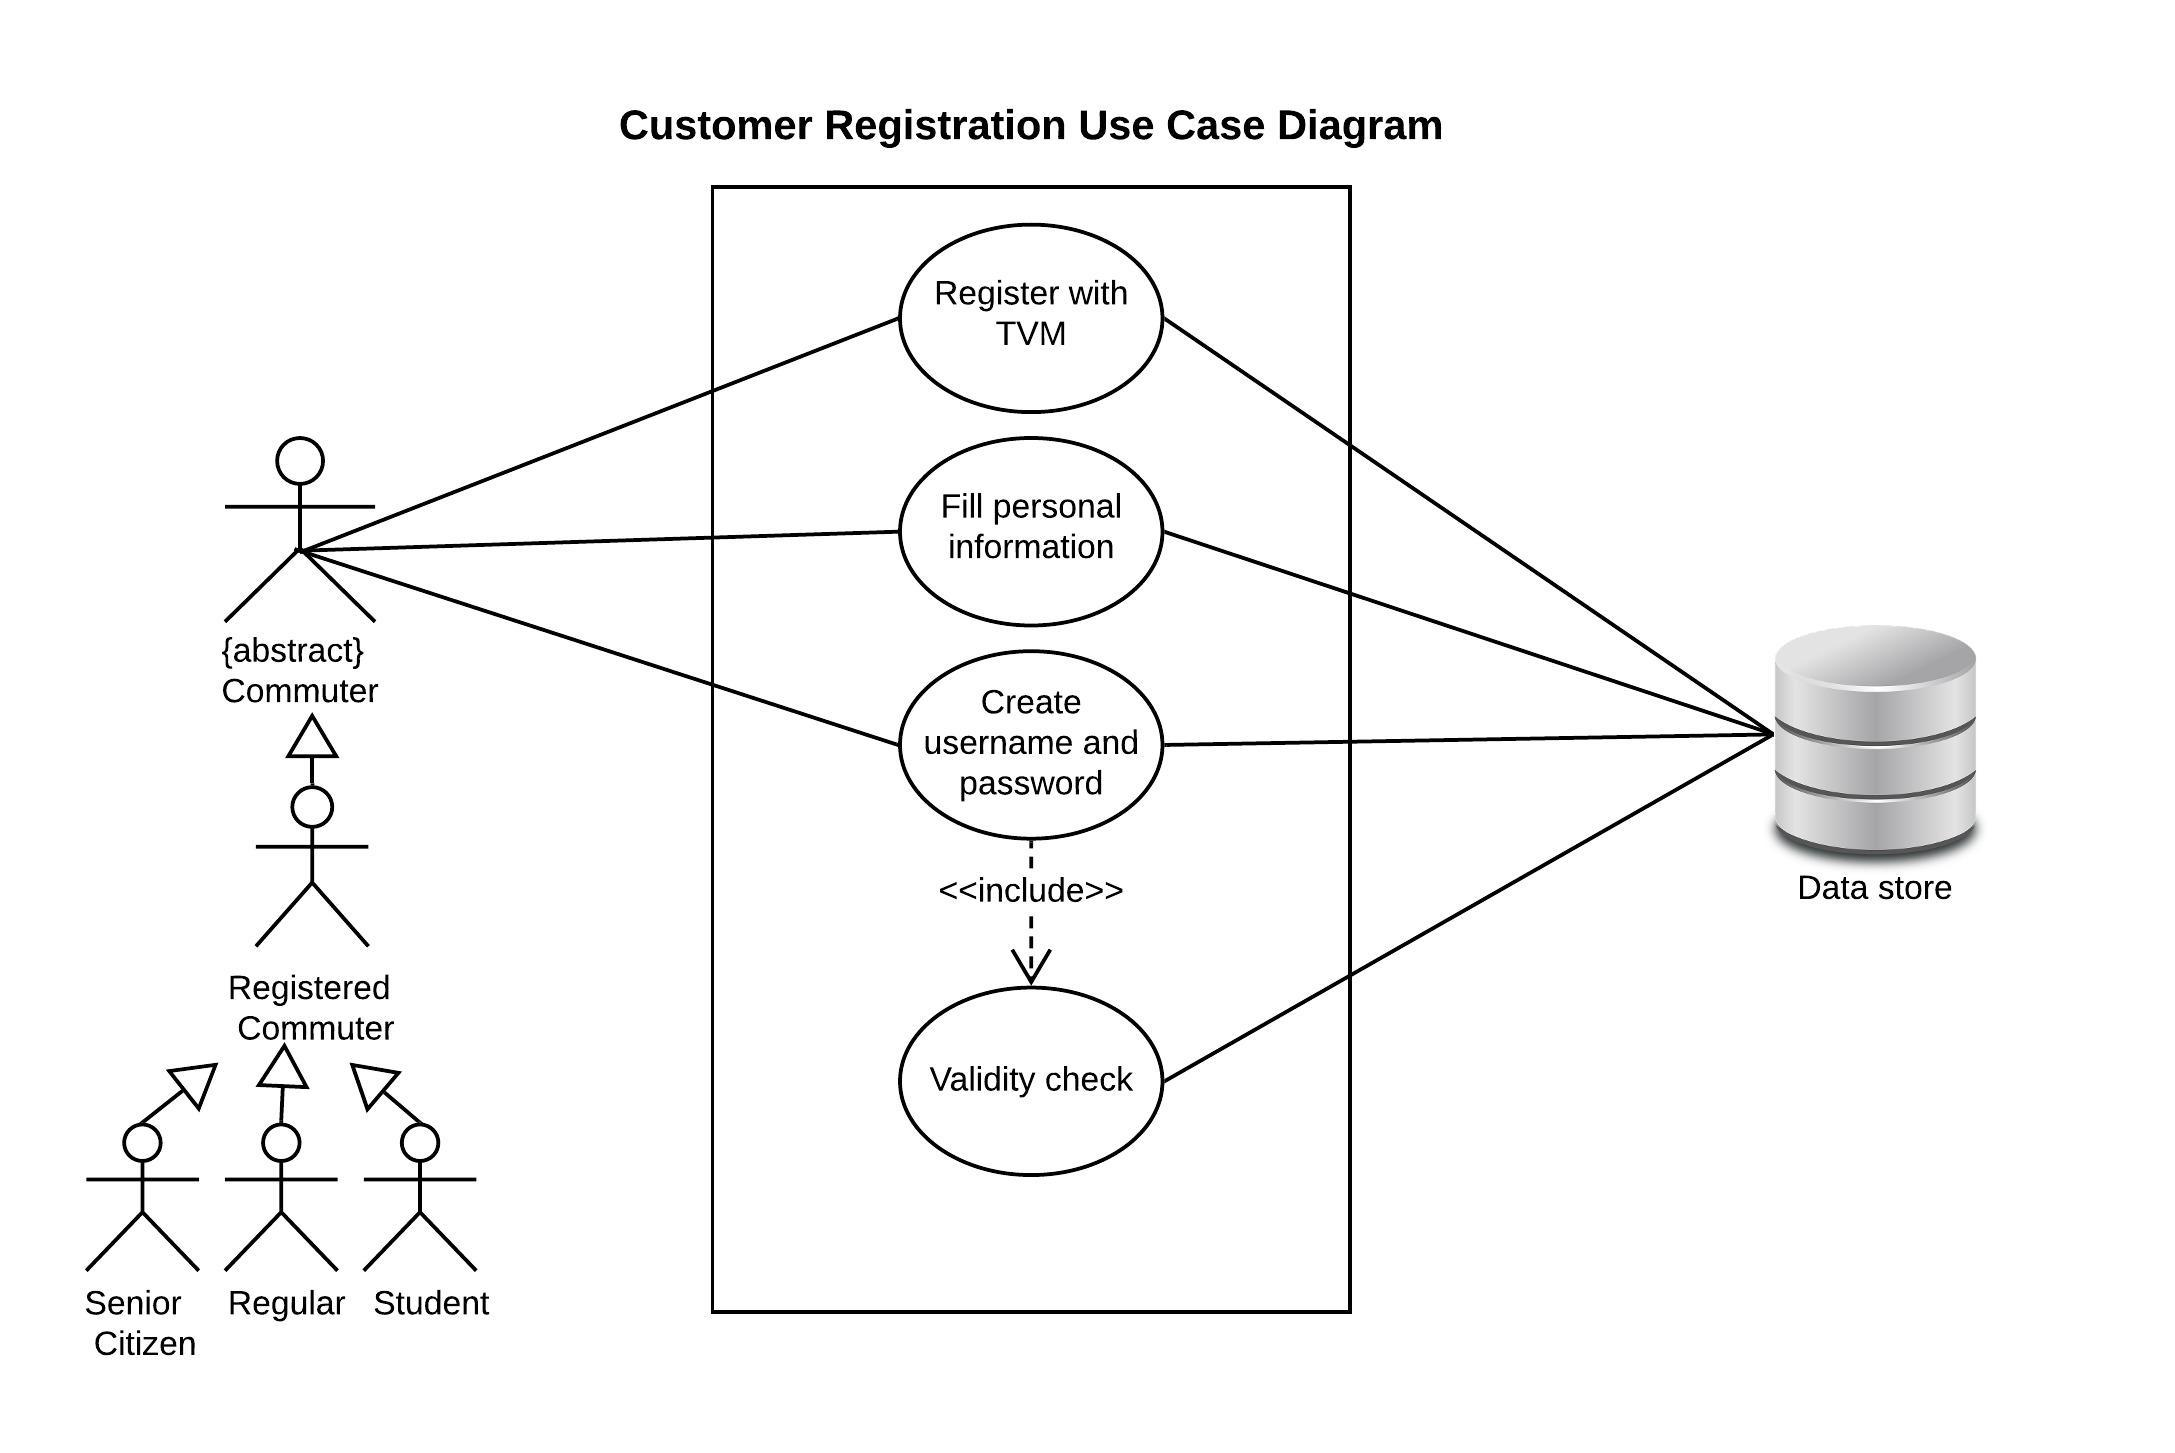
\includegraphics[width=1\textwidth]{Use_Case_Diagrams/CustomerRegistration.jpeg}
	\caption{\label{fig:Use Case Model : } Customer Registration}	
\end{figure}




\vspace{0.5cm}
\textbf{\large Use Case: False Login}
\\

\begin{tabular}{ | c | p{2cm} | p{7cm} |}
	
	\hline
	\textbf{Number} & \multicolumn{2}{c|}{7}  \\
	\hline
	\textbf{Name} & \multicolumn{2}{c|}{False Login}  \\
	\hline
	\textbf{Summary} & \multicolumn{2}{c|}{Hacker try to login into someone else account.}  \\
	\hline
	\textbf{Priority} & \multicolumn{2}{c|}{1}  \\
	\hline
	\textbf{Preconditions} & \multicolumn{2}{c|}{N/A}  \\
	\hline
	\textbf{Postconditions} & \multicolumn{2}{c|}{Login should fail with appropriate error message.}  \\
	\hline
	\textbf{Primary Actor(s)} & \multicolumn{2}{c|}{Hacker / TVM.}  \\
	\hline
	\textbf{Secondary Actors(s)} & \multicolumn{2}{c|}{Data Store}  \\
	\hline
	\textbf{Trigger} & \multicolumn{2}{c|}{User account locked after 5 unsuccessful login attempts.} \\
	\hline
	\textbf{Main Success Scenarios} & \textbf{Step} & \textbf{Action} \\
	\hline
	& 1 & Hacker try to login into system. \\ 
	\hline
	&  2  & Hacker enters username and password. \\
	\hline
	&  3  & System will validate user details from database system. \\
	\hline
	&  4  & System decline unauthorized access. System should display appropriate error message. \\
	\hline
	&  5  & System should display appropriate error message. \\
	\hline
	&  6  & Hacker keeps on entering invalid credentials to try to login into someone account. \\
	\hline
	&  7  & System will lock user account after 5 unsuccessful login attempts. \\
	\hline
	& 8 & System should display account locked error message to user. \\
	\hline
	
	\textbf{Extensions} & \textbf{Step} & \textbf{Branching Action} \\
	\hline
	\textbf{Open Issues} &    & NA \\
	\hline
	
\end{tabular}


%\begin{figure}[!htbp]
%	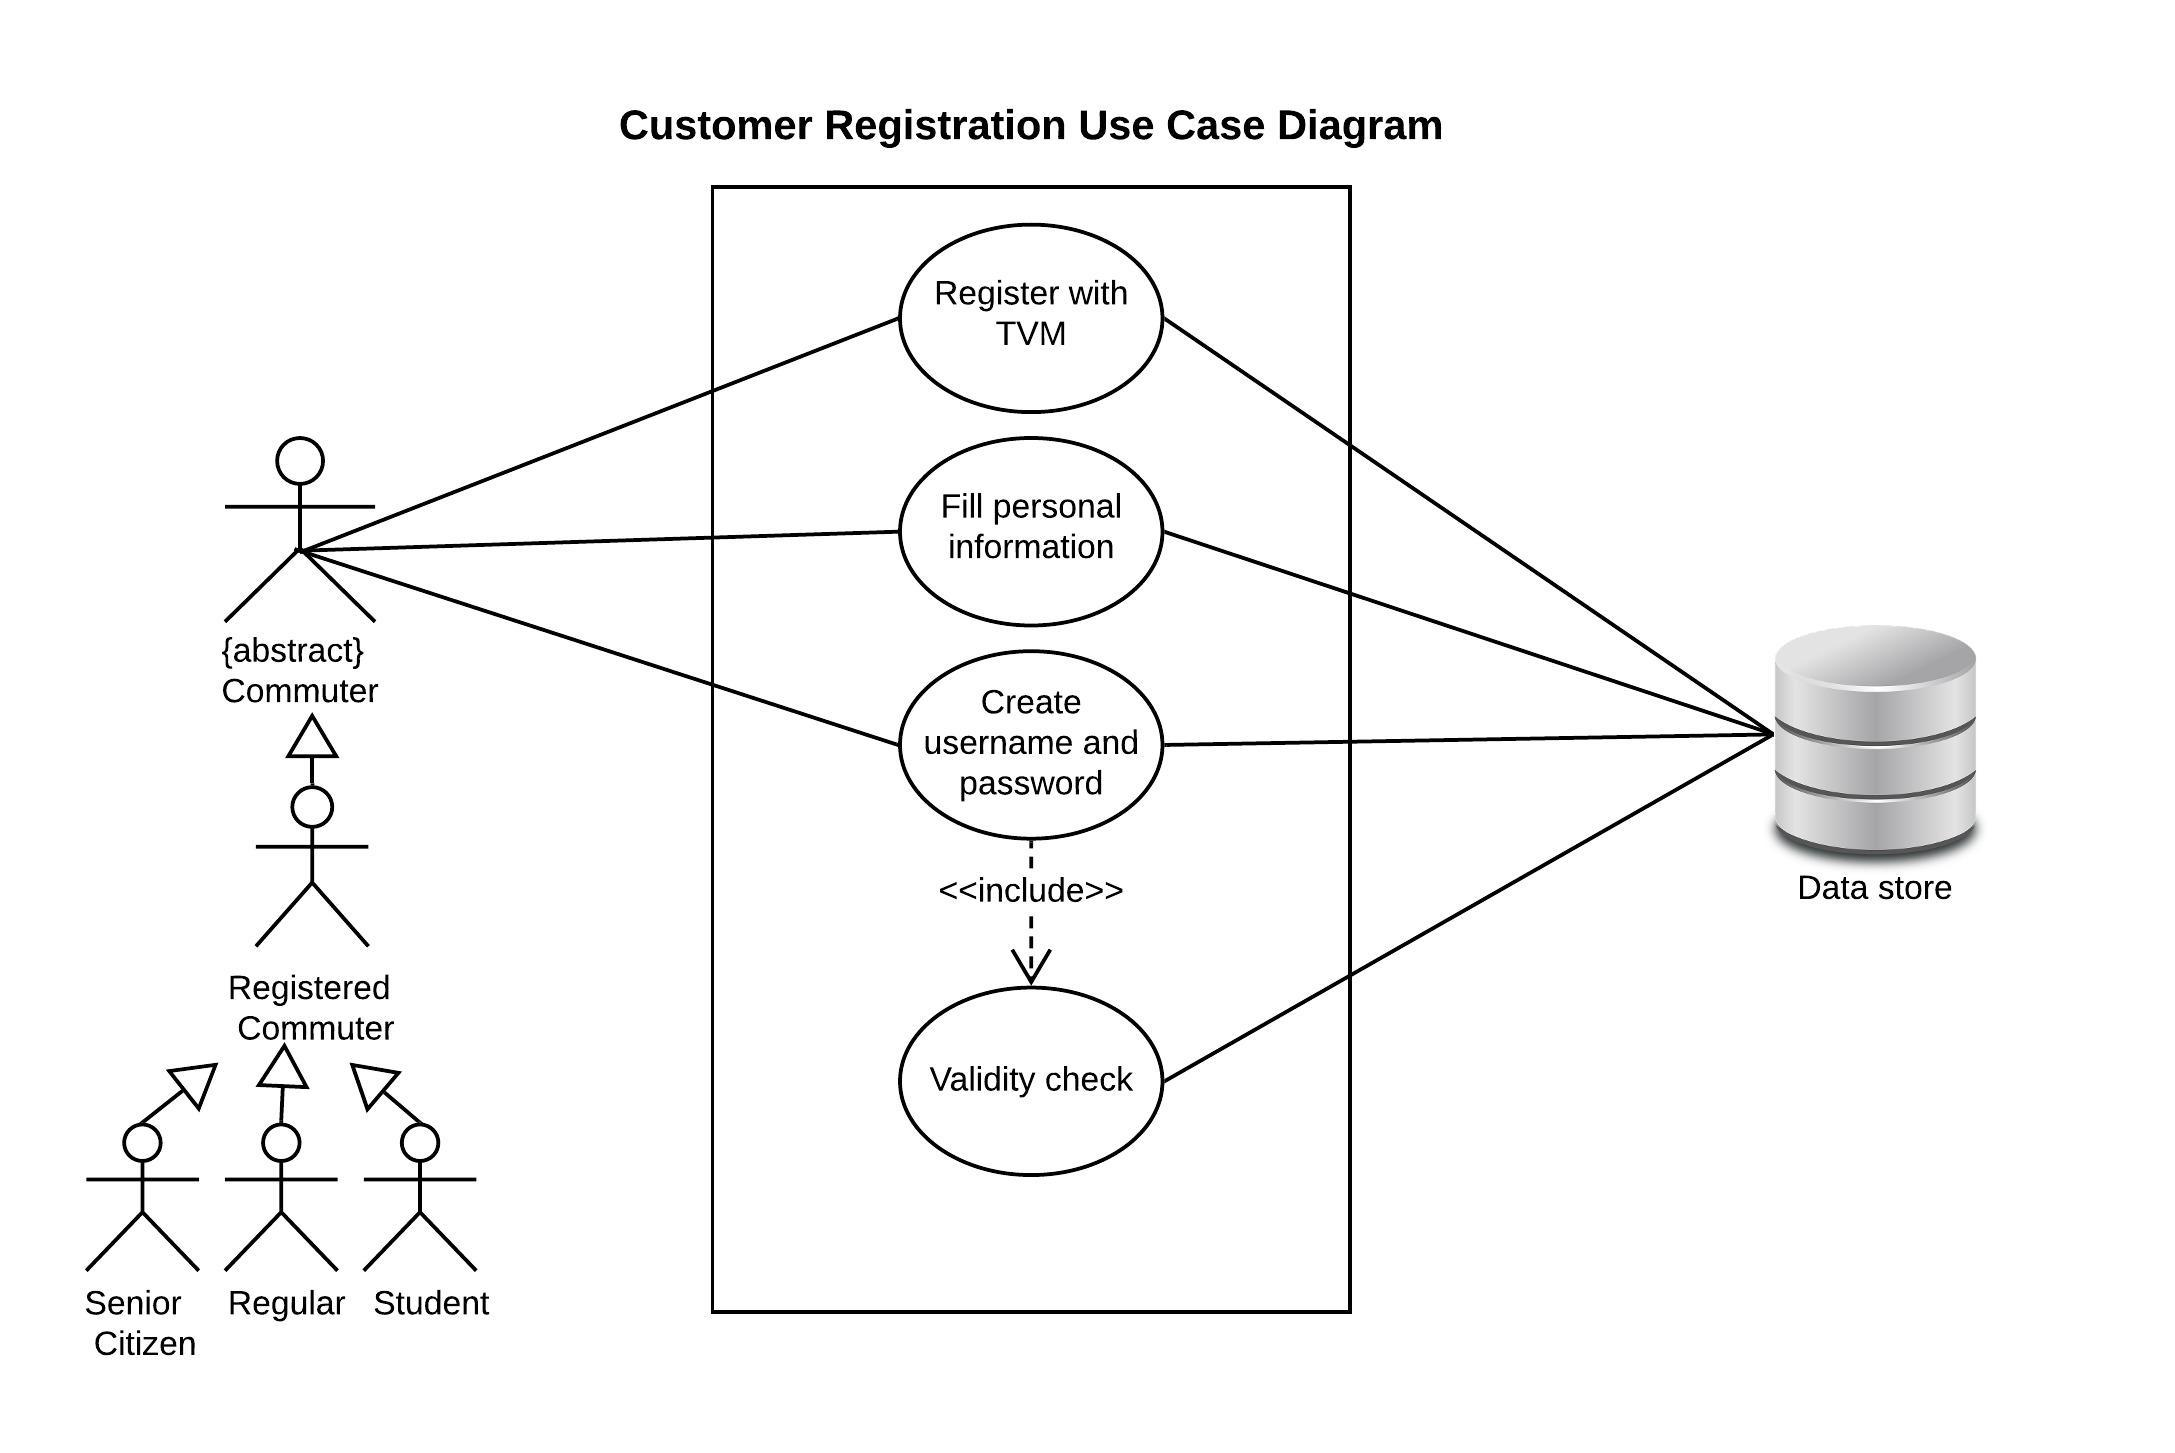
\includegraphics[width=1\textwidth]{Use_Case_Diagrams/CustomerRegistration.jpeg}
%	\caption{\label{fig:Use Case Model : } Customer Registration}	
%\end{figure}



\printglossaries

\end{document}

